%%%%%%%%%%%%%%%%%%%%%%%%%%%%%%%%%%%%%%%%%
% University/School Laboratory Report
% LaTeX Template
% Version 3.0 (4/2/13)
%
% This template has been downloaded from:
% http://www.LaTeXTemplates.com
%
% Original author:
% Linux and Unix Users Group at Virginia Tech Wiki 
% (https://vtluug.org/wiki/Example_LaTeX_chem_lab_report)
%
% License:
% CC BY-NC-SA 3.0 (http://creativecommons.org/licenses/by-nc-sa/3.0/)
%
%%%%%%%%%%%%%%%%%%%%%%%%%%%%%%%%%%%%%%%%%

%----------------------------------------------------------------------------------------
%	PACKAGES AND DOCUMENT CONFIGURATIONS
%----------------------------------------------------------------------------------------

\documentclass{article}

\usepackage[version=3]{mhchem} % Package for chemical equation typesetting
\usepackage{siunitx} % Provides the \SI{}{} command for typesetting SI units
\usepackage{fullpage}
\usepackage{subcaption}
\setlength{\parskip}{3mm}
\usepackage[titletoc,title]{appendix}
\usepackage{xfrac}
\usepackage{tablefootnote}
\usepackage{epstopdf}
\usepackage{enumitem}
\usepackage{etoolbox}
\usepackage{wrapfig}
\usepackage{setspace}
\usepackage{multirow}
\usepackage[bookmarks]{hyperref}
\usepackage{listings}
\patchcmd{\thebibliography}{\section*{\refname}}{}{}{}

\usepackage{graphicx} % Required for the inclusion of images


\usepackage{sourcecodepro}
\usepackage[default]{sourcesanspro}
\usepackage[T1]{fontenc}

\newcommand{\code}{\texttt}

\lstset{
  showspaces=false,
  showtabs=false,
  breaklines=true,
  showstringspaces=false,
  breakatwhitespace=true,
  stringstyle=\color{greenstrings},
  basicstyle=\ttfamily\color{grey}
}

%\setlength\parindent{0pt} % Removes all indentation from 

\renewcommand{\arraystretch}{1.5} % Fix the table sizes
\addtocontents{toc}{\protect\setstretch{-1}}


%\usepackage{times} % Uncomment to use the Times New Roman font

%----------------------------------------------------------------------------------------
%	DOCUMENT INFORMATION
%----------------------------------------------------------------------------------------

\title{\includegraphics[width=.3\textwidth]{/Users/ben/Dropbox/Resources/UVicLogo/UVicLogo} \\ \vspace{7mm} Milestone 2 \\ SENG 310} % Title


\author{UVic Enhancement Suite} % Author name

\date{\today} % Date for the report

\raggedright
\begin{document}

\maketitle % Insert the title, author and date

\begin{center}
\begin{tabular}{l r}
Team Members & Ben Hawker \\
 & Brendon Earl \\
 & Clair Xu \\
 & David Draker \\
 & Kent MacDonald \\
Instructor: & Erini Kalliamvakou  % Instructor/supervisor
\end{tabular}
\end{center}

% If you wish to include an abstract, uncomment the lines below
% \begin{abstract}
% Abstract text
% \end{abstract}

\tableofcontents

%--------------------------------------------------------------------------------
%	RESEARCH METHODS
%--------------------------------------------------------------------------------

\section{Research Methods}

To help guide our design process our team will observe users in a controlled environment to collect qualitative data on how UVic students interact with the current UVic web services, in particular, MyPage and Student Services. After some brief background questions we will ask the students to perform a number of common tasks using the UVic web services.

We believe we can gather more useful information from observing in-person interactions and collecting qualitative data than performing either a quantitative or qualitative survey. Through one-on-one user testing we hope to gain an intuitive insight about how students use UVic web services. Also, in addition to corroborating and prioritizing our current list of pain points, we hope to discover further pain points.

The process used for the user testing is listed in appendix \ref{ap:utesting}.


%--------------------------------------------------------------------------------
%	RESEARCH RESPONSE
%--------------------------------------------------------------------------------

\section{Research Response}

Data is still being analyzed but initial observations have yielded some interesting trends.

\begin{description}
  \item[Calling In] If unable to find the information needed in their web services, many users fall back to calling the department in question.
  \item[Timetable] Most users find their times table but with it was easier to interact with.
  \item[Proof of Enrolment] Many users think that their administrative transcript it the closest thing to a proof of enrolment available from the web services.
  \item[OneCard] Almost all users resort to the search functionality to find their OneCard information.
\end{description}



%--------------------------------------------------------------------------------
%	PERSONAS
%--------------------------------------------------------------------------------
\section{Personas}


\subsection{Junior Student --- Daniel}

\begin{tabular}{lll}
     \multirow{3}{*}{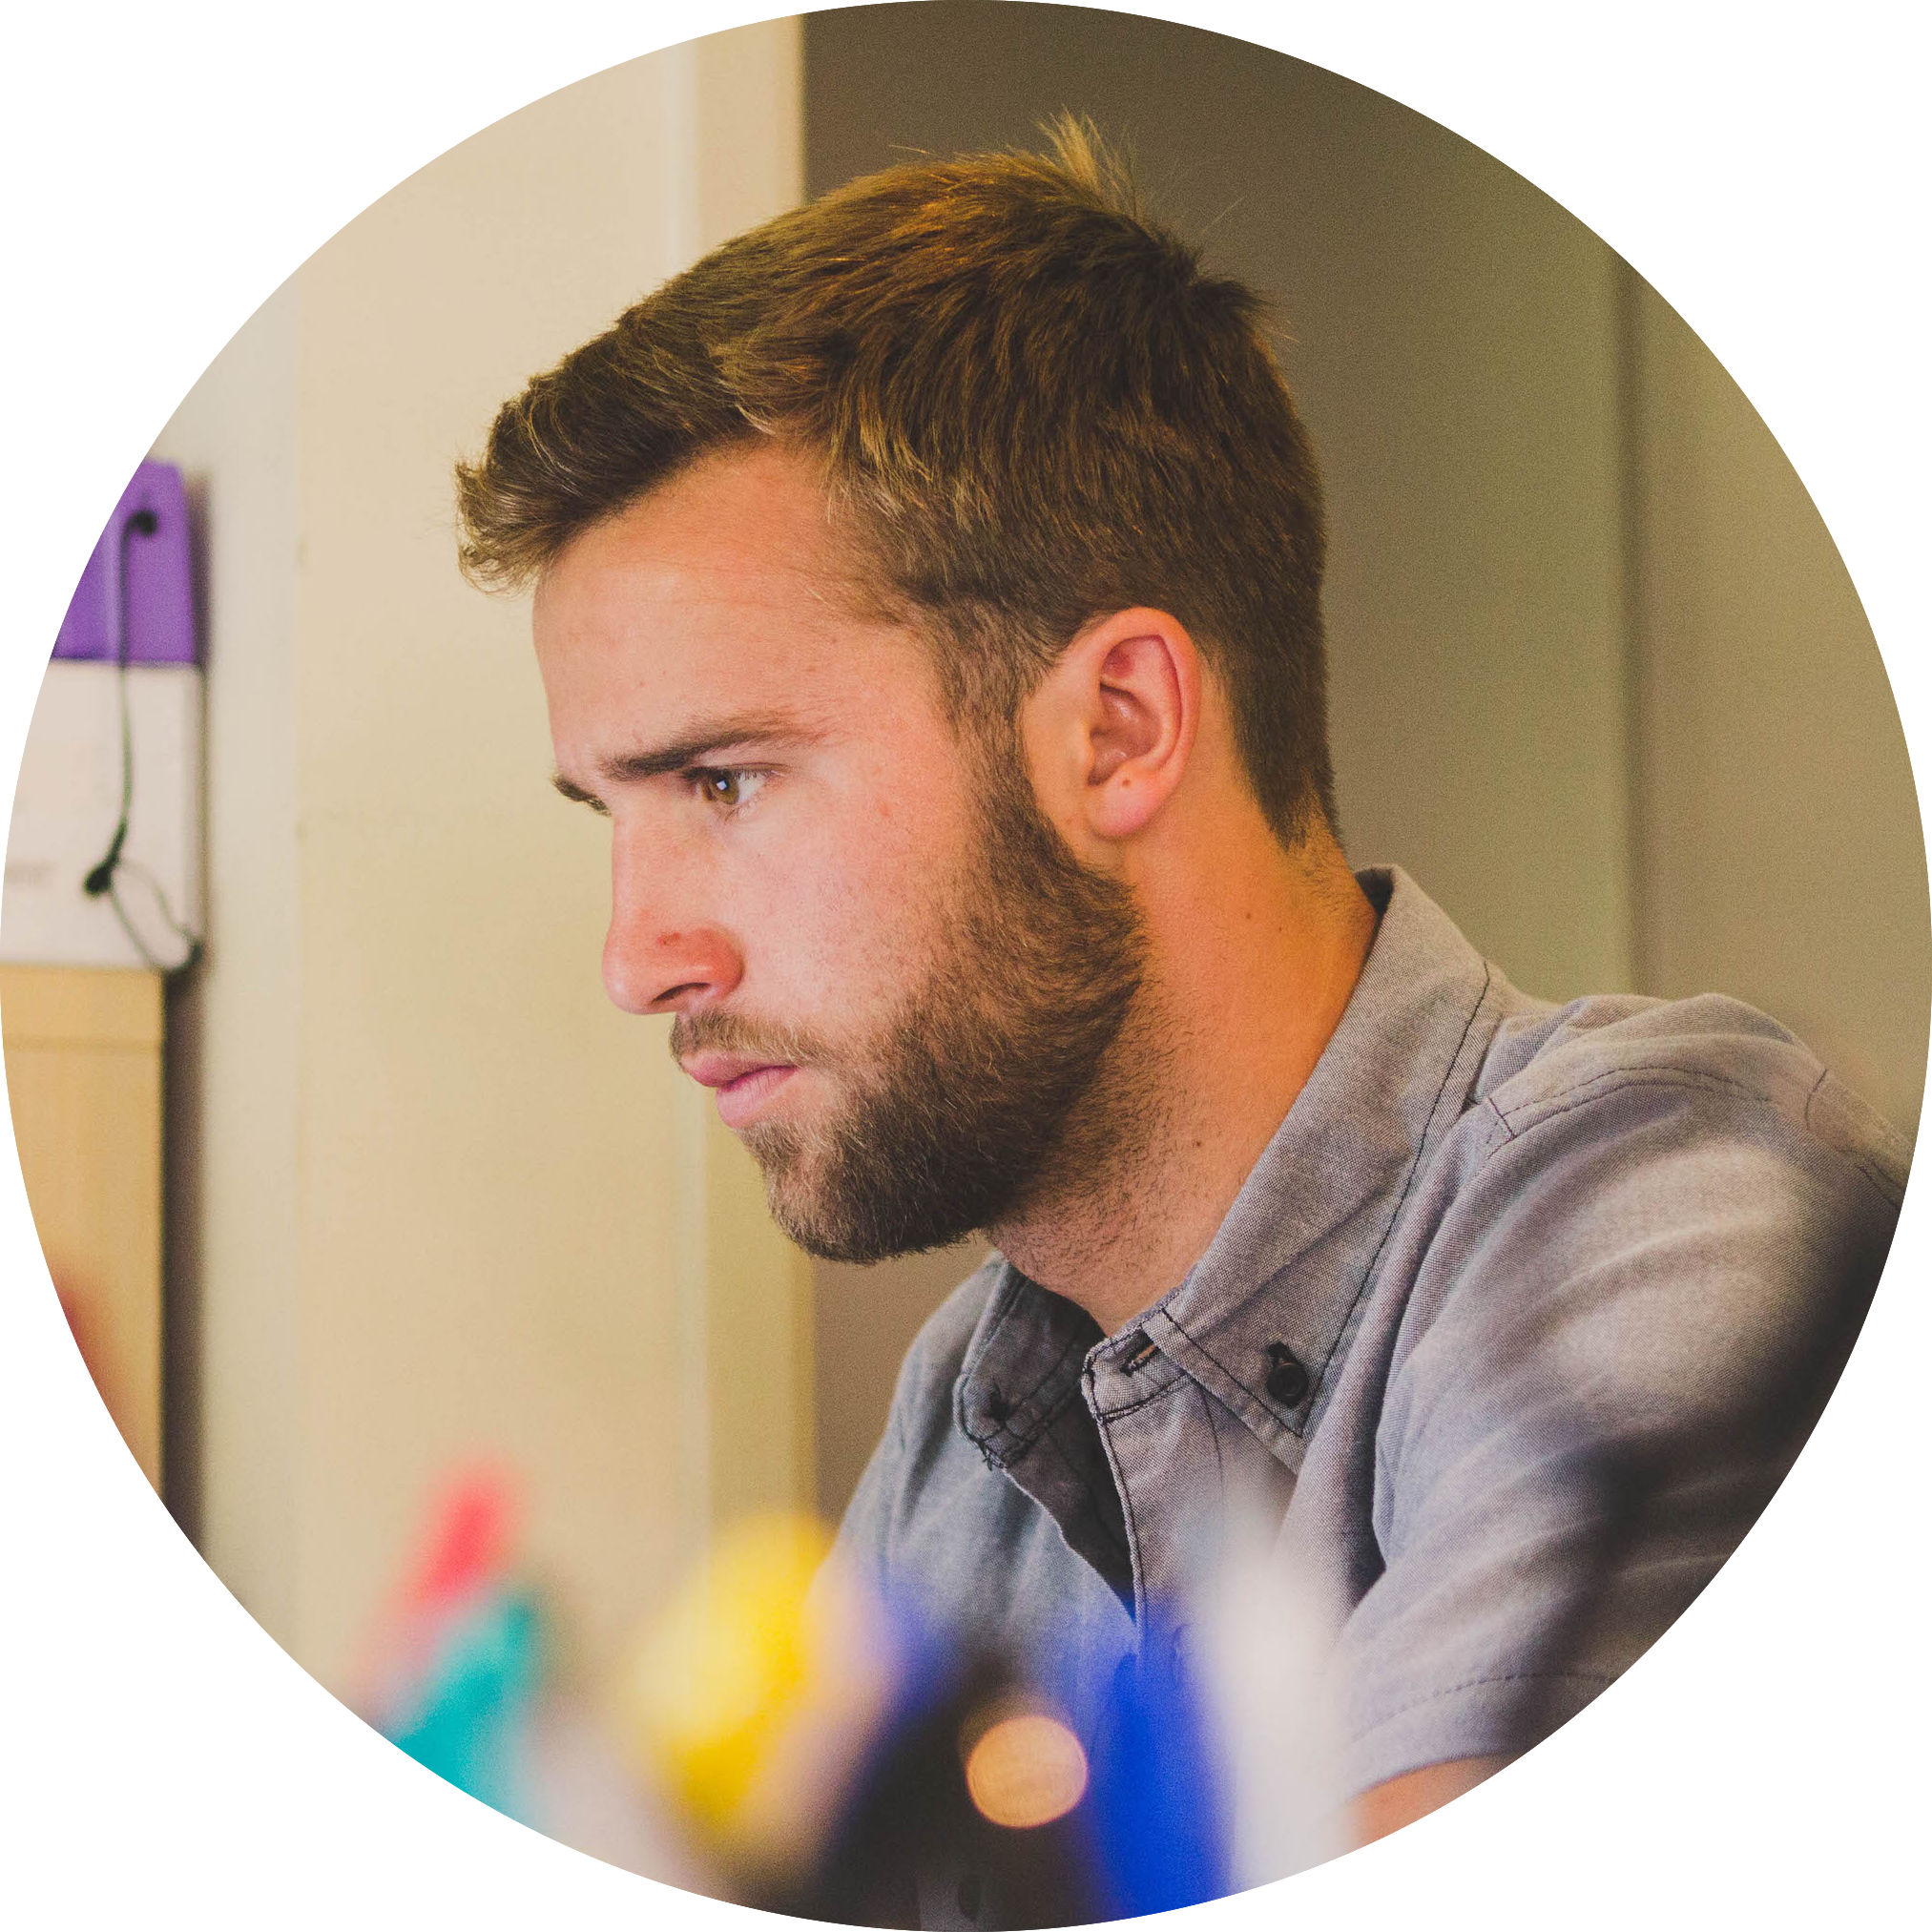
\includegraphics[width=0.12\textwidth]{img/daniel}} & \textbf{Name} & Daniel L\'evesque \\
    & \textbf{Degree} & Earth and Ocean Science \\
    & \textbf{Age} & 22 \\
\end{tabular}


\begin{description}[leftmargin=\parindent,labelindent=\parindent]
    \item[Demographics] Houston, Texas, High School, Christian

    \item[Background] Daniel is a smart, caring, but cautious man from Houston, Texas. He caries forth his southern hospitality to everyone he meets, making him an easy man to get along with. After graduating from high school he stayed in his hometown to look after his family and sick grandmother. Working an evening job as a carpenter, he helped out with his family of 3 sisters and 2 brothers, 3 of which under the age of 12, by driving, running errands, and cooking food - after all, he was the eldest and assumed responsibility when his father passed away.
    
    Four years after graduating, his grandma passed and with his siblings getting older, he decided to take a step forth in his life and get a degree in Earth and Ocean Sciences. Given the times he spent at the beach and lay in awe as the waves crash, or when a storm hits and the wind whips, he was fascinated in the science behind it all. UVic provided him with the program he wants and the lush greenery and coastal environment he so desired, and so his first week begins today.
    
    \item[Habits]~\\
    
    \begin{itemize}
        \item Desktop (PC), Mobile (Android)
        \item Microsoft Office, Twitter
        \item Sketching
        \item Reading
    \end{itemize}

\end{description}

\subsection{Senior Student --- Amy}

\begin{tabular}{lll}
    \multirow{3}{*}{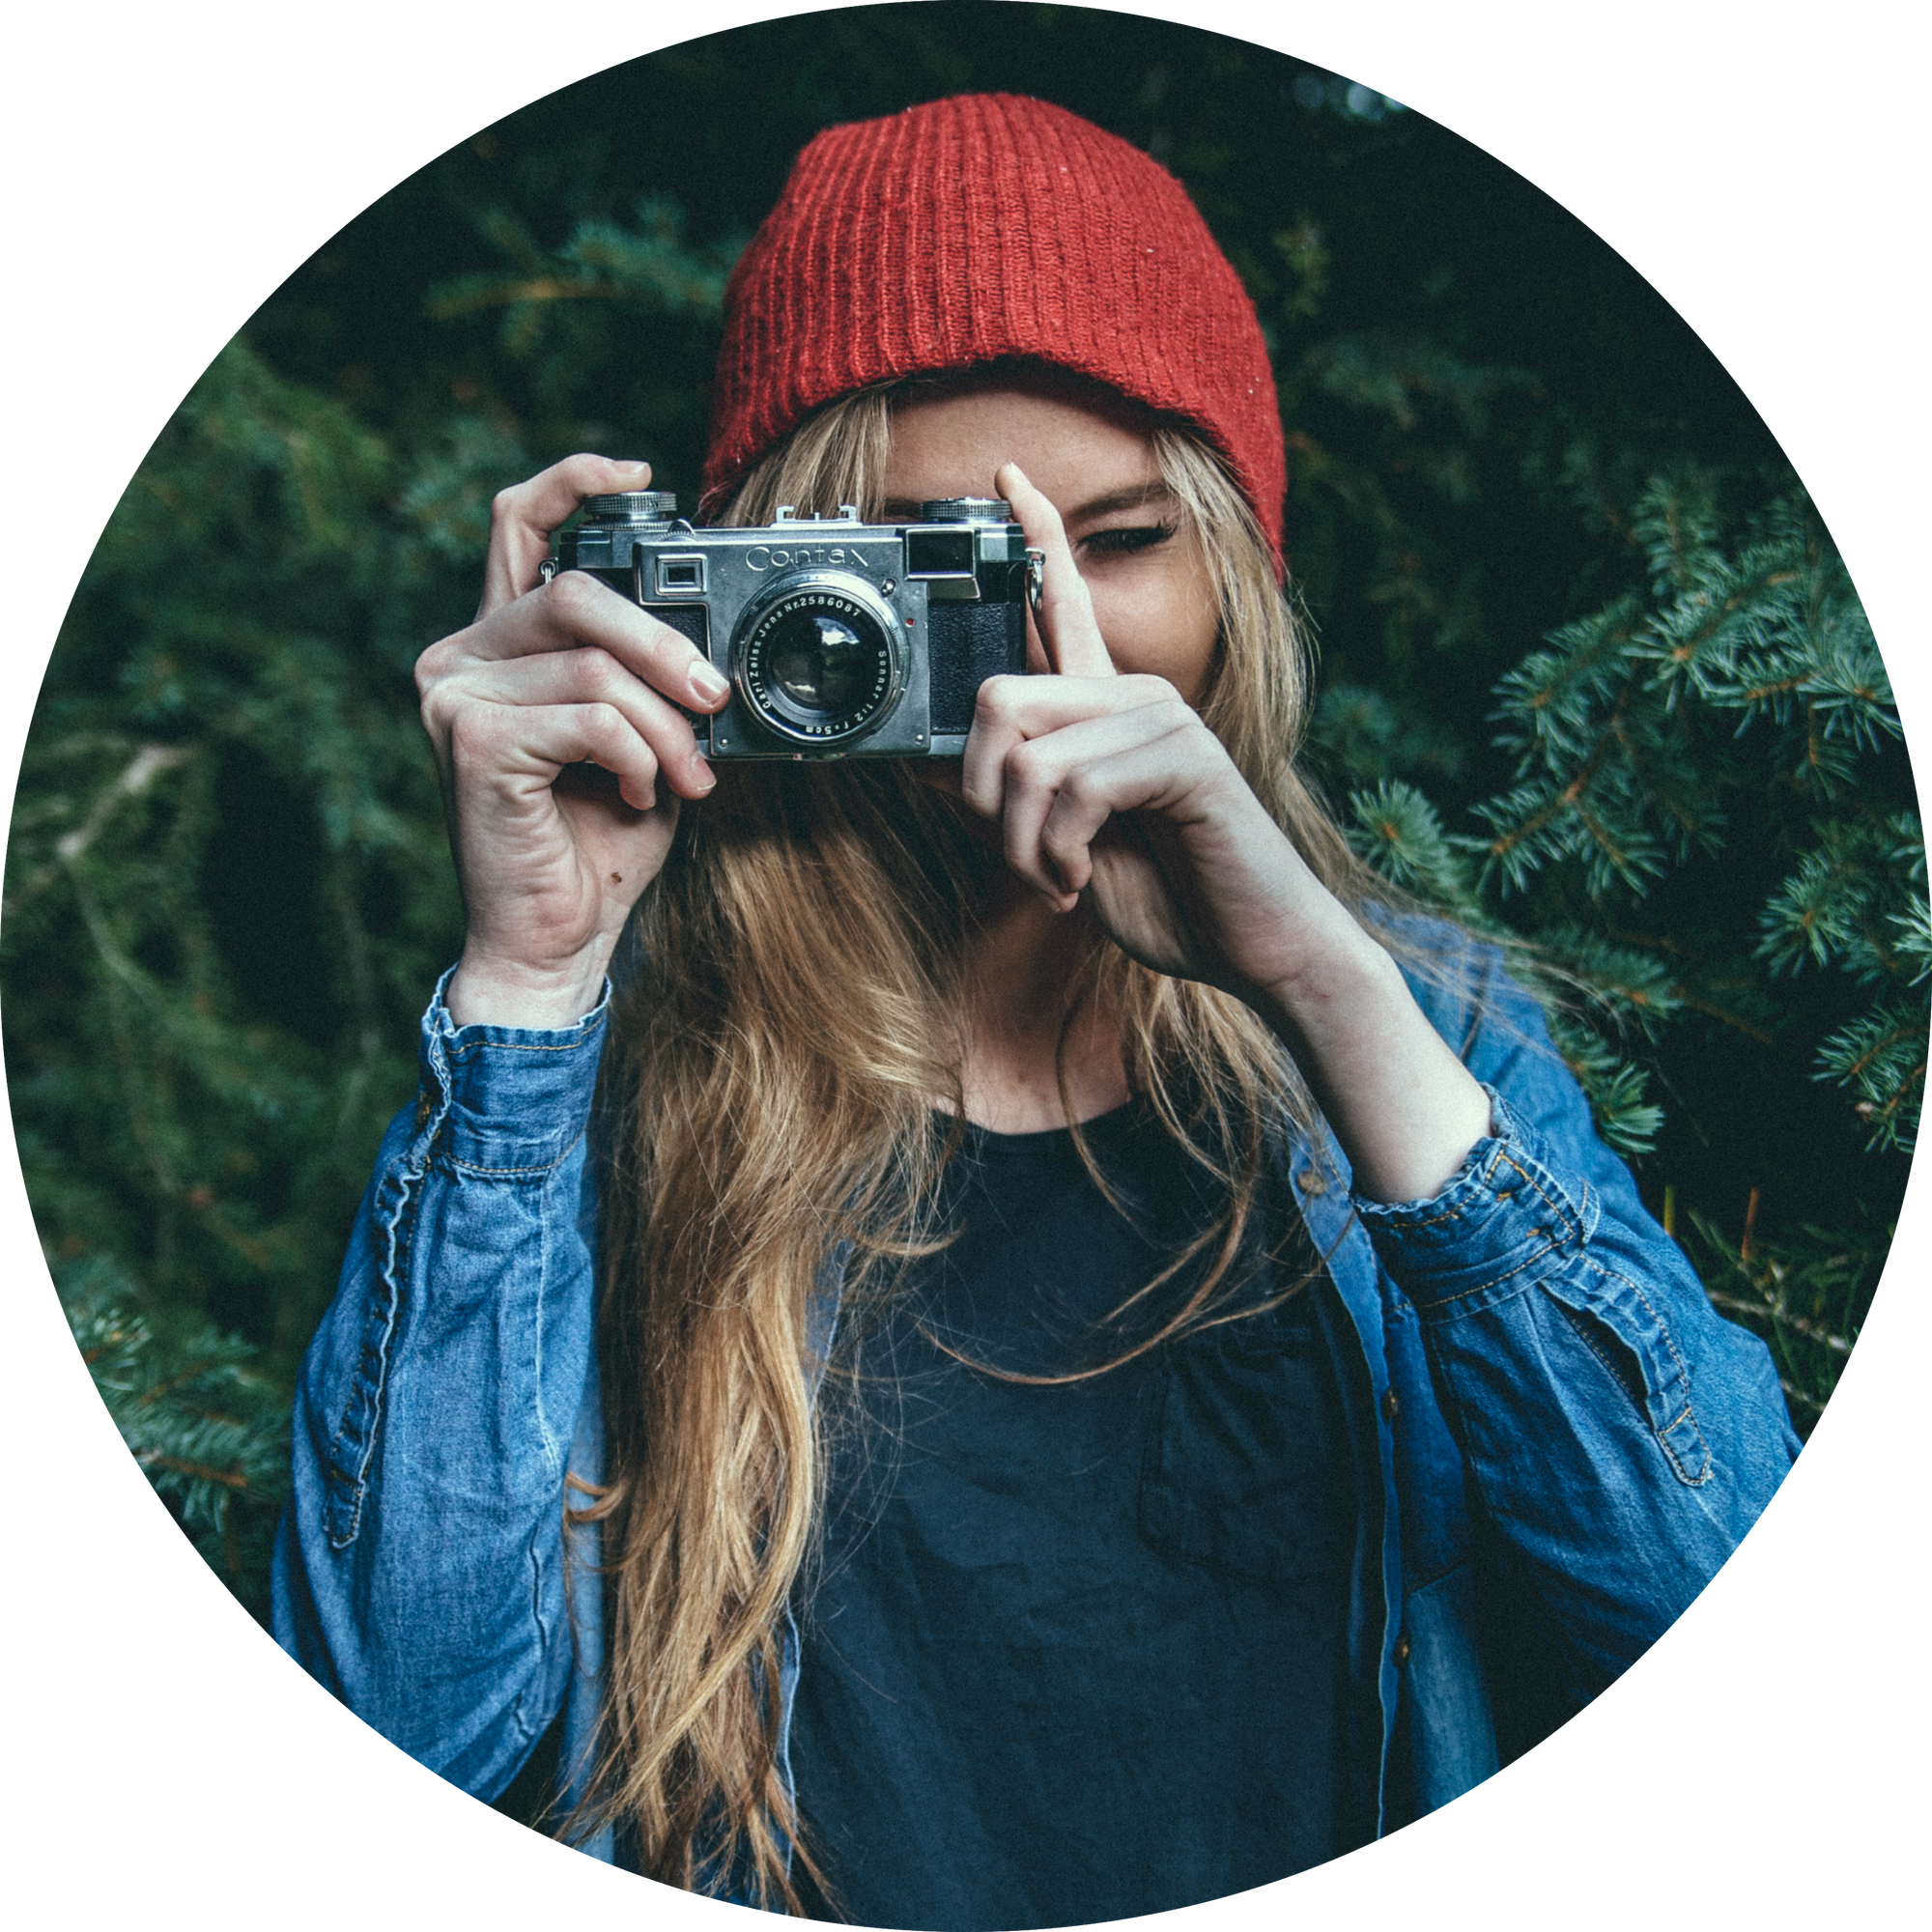
\includegraphics[width=0.12\textwidth]{img/amy}} & \textbf{Name} & Amy Bailey \\
    & \textbf{Degree} & Film Studies \\
    & \textbf{Age} & 35 \\
\end{tabular}

\begin{description}[leftmargin=\parindent,labelindent=\parindent]
    \item[Demographics] Fredericton, New Brunswick, Digital Filmmaking Professional Diploma, Buddhist

    \item[Background] Amy is an artsy 35 year old girl from Fredricton, New Brunswick. After graduating from high school she decide to travel. After visiting places such as Morocco, Cuba, Peru, and Nicaragua, she fell in love with the many stories told to her by locals along her trip and the unique dance at each location. Inspired by people of the world's ability to express themselves, Amy set out to capture her perspective and tell stories.  

    Once home in Canada, Amy attended the Centre for Arts and Technology in her hometown, Fredericton. After completing the 12 month program, she began filmmaking with a few friends she met while travelling and later formed a film company. Together they produced short films  and documentaries on cultures around the world, earning a position as some of the best documentaries at film festivals due to their wide perspective and deep understanding of their field.
    
    After many years of film producing, Amy is taking her production and company to the next level by getting a degree in Film Studies at UVic. What drove her here was the freedom a new part of the country presented, while still providing a coastal atmosphere. In her third year of study she's digging deeper into relevant courses, while also beginning to see the light at the end of the tunnel - and developing valuable ideas as a result. As effective as Amy has been producing films, she can be a bit forgetful at times when her creativity takes over. 
    
    \item[Habits]~\\
    
    \begin{itemize}
        \item Mobile (iPhone), Laptop (Macbook)
\item Microsoft Office, Adobe Lightroom, Instagram 
\item Editing photos, making documentaries
\item Hiking, Snowshoeing
    \end{itemize}

\end{description}

\pagebreak
\subsection{International Student --- Seoyeon}

\begin{tabular}{lll}
    \multirow{3}{*}{\includegraphics[width=0.12\textwidth]{img/seoyeon}} & \textbf{Name} & Seoyeon Song \\
    & \textbf{Degree} & Environmental Studies \\
    & \textbf{Age} & 21 \\
\end{tabular}

\begin{description}[leftmargin=\parindent,labelindent=\parindent]
    \item[Demographics] Seoul, South Korea, Shopping

    \item[Background] Seoyeon is a 21 year old international student who is currently studying Environmental Studies at the University of Victoria. Seoyeon comes from a culture significantly different from Western culture -- Seoul, South Korea. Compared to native students, Seoyeon takes more time to read things written in English, as she tend to translate everything into Korean in her mind to help herself understand it better.

    Most Environmental Studies classes go to the field often, so her lectures are always in different locations. Seoyeon has to check her timetable and Coursespaces often to figure out where she needs to go for her next class. However, it always takes many clicks to get to her weekly timetable. She would like an easier way to find out where she has to go for her next class.
    
    \item[Habits]~\\
    
    \begin{itemize}
        \item Desktop (Macbook), Mobile (Android)
        \item Reading
        \item Observing plants
        \item Shopping
        \item Watching Korean TV shows
    \end{itemize}

\end{description}

%--------------------------------------------------------------------------------
%	SCENARIOS
%--------------------------------------------------------------------------------

\section{User Stories}

\subsection{Scholarship Application}

Amy, like many other university students is starting to run out of money by her 3rd year of university. She decides to apply for a few scholarships. After spending a few hours on one of the applications, the form says to attach a copy of his "Official Transcript" and "Summary of Tuition Fees". Lucius spends the rest of his night attempting to find these documents on the UVIC myPage website. Unfortunately, due to the confusing layout of the website he was unsuccessful, and unable to submit the application.

\subsection{First Class}

It's Tuesday, Daniel has just started his first semester of classes at UVic. He needs to get to his first class, MATH 100. He finds the course on his timetable but doesn't know what DTB is. He finds out it's the David Turpin Building from the website but then someone says to "just go to SSM" and he gets confused. Not sure where his class is Daniel ends up in the David Strong Building and sits through a full hour and twenty minutes of ECON 103c.



%--------------------------------------------------------------------------------
%	Appendices
%--------------------------------------------------------------------------------
\pagebreak
\begin{appendices}

\section{User Testing Plan}\label{ap:utesting}

\subsection*{Introductory Questions}\label{introductory-questions}
\subsubsection*{Personal}\label{personal}
\emph{What's your name?} \\
\emph{Where are you from?} \\
\emph{How many years have you been at UVic?} \\
\subsubsection*{UVic Website Questions}\label{uvic-website-questions}
\emph{When was the last time you were on the UVic website?} \\
\emph{What were you there for?} \\
\emph{Did you find it okay?} \\
\emph{What is the most common reason you go to the UVic website?} \\
\subsection*{Tasks}\label{tasks}
\subsubsection*{Finding a Class}\label{finding-a-class}
\emph{What class do you have next? What's the professor's name?} \\
\subsubsection*{Finding Account Information}\label{finding-account-information}
\emph{How much tuition did you pay three semesters ago?} \\
\subsubsection*{Finding Forms}\label{finding-forms}
\emph{Can you get your proof of enrolment?} \\
\emph{Can you get your T2202a?} \\
\subsubsection*{Finding OneCard Information}\label{finding-onecard-information}
\emph{What is your OneCard balance?} \\
\subsection*{Closing Questions}\label{closing-questions}
\emph{Was there anything you found particularly difficult?} \\
\emph{Is there anything you think we missed?} \\

\pagebreak
\subsection*{User Testing Consent Form}\label{ap:ut-consent}

\begin{center}
    \textbf{Consent Form for Participation in \\ UVic Web Services User Testing}
\end{center}

You are being invited to participate in user testing of the UVic web services that is being conducted by the UVic Enhancement Suite Team, and you may contact Ben Hawker if you have further questions at bhawker@uvic.ca.

You will be asked some introductory questions about the UVic web services and asked to perform some tasks relating to your web services. You will also be asked for some demographic information (age, occupation, etc.). Your participation should require about 30 minutes of your time. The results will be reported in a project report for SENG 310 in the Faculty of Engineering at the University of Victoria.

Your participation is completely voluntary and you can withdraw from the study at any time, without explanation. You have the right to refuse to answer any questions you do not wish to answer.

Any data collected in the study will remain confidential. Only the principal and co-investigators will have access to the data. Your name will not be attached to any published results, and your anonymity will be protected by using code numbers to identify results obtained from individual subjects.

With your consent, your interview will be audiotaped to be referred to later by the investigators.

Whether you participate or choose not to participate will have no bearing on your grade/employment status/academic standing/job/services received.

\begin{center}
    \textit{Signatures}
\end{center}

\emph{\textbf{A copy of this consent will be left with you, and a copy
will be taken by the researcher.}}


\end{appendices}


%--------------------------------------------------------------------------------
%	BIBLIOGRAPHY
%--------------------------------------------------------------------------------

%\section{References}
%
%\bibliographystyle{unsrt}
%



%--------------------------------------------------------------------------------

\end{document}